Le modèle PetriNet que j'ai utilisé est représenté par le diagramme suivant :

\begin{center}
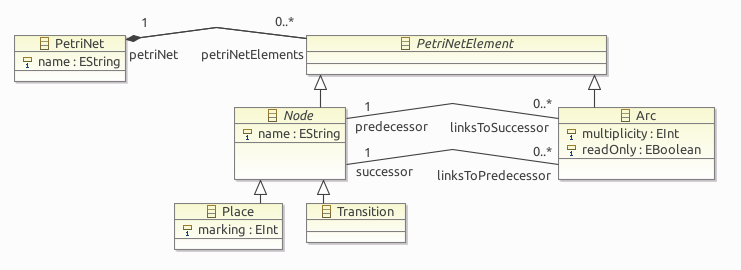
\includegraphics[width=\textwidth]{../Images/meta_petri.png}
\end{center}



Ce modèle n'est pas suffisant pour décrire entièrement l'ensemble des contraintes. Pour celà on a donc ajouté des contraintes OCL avec OCLinEcore.\\

On a ajouté les règles suivantes :
\begin{itemize}
\item class PetriNet
\begin{itemize}

\item voidPetriName : nom vide interdit
\item sameNodeName : les noms des noeuds doivent être différents
\end{itemize}

\item abstract class Node
\begin{itemize}
\item voidNodeName : nom vide interdit
\end{itemize}

\item class Arc
\begin{itemize}
\item positiveMultiplicity : la multiplicité doit être > 0
\item sameTypeOfPredecessorAndSuccessor : Prédecesseur et successeur doivent être différents
\item nextNodeNotInSamePetriNet : les noeuds reliés sont dans le même réseau de pétri
\item previousNodeNotInSamePetriNet :les noeuds reliés sont dans le même réseau de pétri
\end{itemize}

\item class Place
\begin{itemize}
\item positiveMarking : le marquage d'une place est >= 0
\end{itemize}
\end{itemize}
